\documentclass[11pt,a4paper]{article}
\usepackage[utf8]{inputenc}
\usepackage[T1]{fontenc}
\usepackage[brazil]{babel}
\usepackage{lmodern}
\usepackage{amsmath,amssymb,bm}
\usepackage{graphicx,booktabs,float,geometry,url,pdflscape,longtable,array,xcolor}
\usepackage[hidelinks]{hyperref}
\geometry{margin=2.2cm}
\emergencystretch=2em
\setlength{\LTcapwidth}{\linewidth}
\providecommand{\versao}{sem versão}
\newcommand{\gw}{\gamma_w}
\newcommand{\tl}{\textbackslash}
% gerado por figuras_contornos.py; nao edite a mao
\newcommand{\tabdominio}{%
\begin{tabular}{lrrrr}\toprule
Domínio (atrás da crista; à frente do pé; abaixo do pé) & A & B & C & D \\ \midrule
notebook (3,5H; 3H; 3H) & 1{,}409 & 1{,}382 & 1{,}268 & 1{,}260 \\
nosso domínio (7H; 6H; 6H) & 1{,}400 & 1{,}393 & 1{,}329 & 1{,}322 \\
Fig.~4 aprox.\ (13H; 2H; 8H) & 1{,}361 & 1{,}433 & 1{,}400 & 1{,}328 \\
\bottomrule\end{tabular}}
\newcommand{\tabinstantaneo}{%
\begin{tabular}{llrrr}\toprule
Água & $t$ (h) & $\Gamma$ GIM u-pw-pa & $\Gamma$ GIM u-p & $\Gamma$ cinemático \\ \midrule
saturada & 0+ & 0{,}489 & 0{,}489 & 0{,}543 \\
saturada & 0,1 & 2{,}583 & 2{,}583 & 2{,}308 \\
saturada & 1 & 8{,}182 & 8{,}182 & 3{,}673 \\
saturada & 10 & 8{,}369 & 8{,}369 & 3{,}706 \\
não saturada & 0+ & 0{,}489 & 0{,}489 & 0{,}543 \\
não saturada & 0,1 & 1{,}398 & 1{,}398 & 1{,}341 \\
não saturada & 1 & 1{,}541 & 1{,}541 & 1{,}477 \\
não saturada & 10 & 1{,}698 & 1{,}698 & 1{,}602 \\
\bottomrule\end{tabular}}
\newcommand{\gcin}{1{,}342}
\newcommand{\gextceron}{1{,}340}
\newcommand{\gextres}{1{,}279}
\newcommand{\gcerii}{1{,}484}
\newcommand{\gceriii}{1{,}401}
\newcommand{\gceriv}{1{,}366}
\newcommand{\gcerv}{1{,}351}
\newcommand{\gdetii}{1{,}396}
\newcommand{\gpyfino}{1{,}323}
\newcommand{\gpzufino}{1{,}327}
\newcommand{\dufino}{0{,}54}

\title{Os contornos da água no rebaixamento e na chuva:\\ Ceron (2025), o PZ e Rahardjo et al.\ (2007)}
\author{Diogo Cecílio}
\date{20/11/2026 --- versão \versao}
\begin{document}
\maketitle
\begin{abstract}
O nosso Monte Carlo do rebaixamento dá $P_f = 15{,}7\,\%$; o Ceron (2025) dá $11{,}5\,\%$ no mesmo problema. Este
documento junta, num lugar só, as condições de contorno da água de cada análise: o Ceron (como está no artigo e como
identificamos pela Fig.~4b), o PZ com o contorno \texttt{reservatorio} (o do nosso MC) e com o contorno
\texttt{ceron} (novo), e a chuva do Rahardjo como está no código. Cada contorno tem um esquema em escala
(Figuras~\ref{fig:a} a \ref{fig:e}) e uma linha numa tabela (Tabelas~\ref{tab:unica} e \ref{tab:rahardjo}). Os
resultados já obtidos mostram que a água pesa mais que o método: com a água do Ceron, o PZ dá
$\Gamma = \gextceron$ (extrapolado) e o método cinemático dá $\gcin$, contra $1{,}336$ do artigo; com a nossa água de
0,1~h, o PZ dá $\Gamma \approx 1{,}28$. Os próximos passos são o MC com a água do Ceron (em Python e no PZ) e, depois,
a chuva.
\end{abstract}
\tableofcontents

\section{Por que o contorno da água decide a $P_f$}
\begin{itemize}
  \item \textbf{A discrepância (etapa 3d do README):} o nosso MC direto do rebaixamento (2000 realizações, GIM, 3 níveis
    de refinamento) dá $P_f = 15{,}70\,\%$ (IC de 95\,\%: 14,1 a 17,3\,\%); o Ceron dá $11{,}50\,\%$
    ($\mathrm{CoV} = 2{,}77\,\%$). A diferença é de uns 5 desvios.
  \item \textbf{O método não explica:} na mesma água, o método cinemático (o do Ceron, refeito em Python em
    \path{Projects/CeronCinematico}) e o GIM extrapolado do PZ diferem 0,3\,\% no determinístico.
  \item \textbf{A água explica:} o Ceron usa percolação \emph{permanente} saturada logo depois do rebaixamento
    instantâneo (Eqs.~19--21 do artigo); nós usamos um transiente de 0,1~h com outros contornos. Só mudando os
    contornos da água permanente, o $\Gamma$ do mesmo talude vai de 1,26 a 1,43 (Seção~\ref{sec:dominio}).
  \item \textbf{O objetivo:} (1) validar o Ceron, chegando a $P_f \approx 11{,}5\,\%$ com a água dele; (2) depois,
    resolver a chuva do Rahardjo no transiente u-pw-pa com contornos que sabemos justificar.
\end{itemize}
A formulação da água não saturada está em \path{docs/nao_saturado}; a dos campos aleatórios e do MC, em
\path{docs/confiabilidade_campos/formulacao}. Aqui só aparecem os contornos e os números.

\paragraph{Notação.} $u$ é o \emph{excesso} de poropressão: $u = p - \gw y$ no Ceron, com $y$ para baixo a partir da
crista. No PZ, $y$ aponta para cima e a crista fica em $y = 35$, então $u = p_w - \gw(35 - y)$. Nas figuras usamos a
origem na aresta da crista e a cota para cima. $H = 5$~m, $\beta = 45^\circ$ e o nível final fica no pé ($h_w = H$).

\section{Os contornos em figuras}\label{sec:esquemas}
As cores são as mesmas em todos os esquemas: azul, $u = 0$ (hidrostática com o nível na crista, ou do NA no
Rahardjo); laranja, $u = -\gw y$ ($p = 0$ na face); rosa, $u = -\gw h_w$ (hidrostática do nível final); verde
traço-ponto, face de percolação; cinza tracejado, sem fluxo; vermelho, a chuva. Cada trecho também tem o rótulo
escrito.

\subsection*{(a) Ceron (2025)}
O texto do artigo dá só a crista, a face e o pé (Eq.~1 e Eq.~21: $\partial\Omega_{u1}$, $\partial\Omega_{u2}$,
$\partial\Omega_{u3}$) e diz que $\partial\Omega_v = \emptyset$. Laterais e base não aparecem: o domínio da Fig.~2
não tem limites. Reproduzindo a Fig.~4b (Seção~\ref{sec:fig4}), as laterais e a base que batem são: lateral esquerda e
base com $u = 0$ e lateral direita \emph{sem fluxo}. Isso contradiz o ``$\partial\Omega_v = \emptyset$'' literal, que
pediria $u$ imposto também à direita.
\begin{figure}[H]\centering
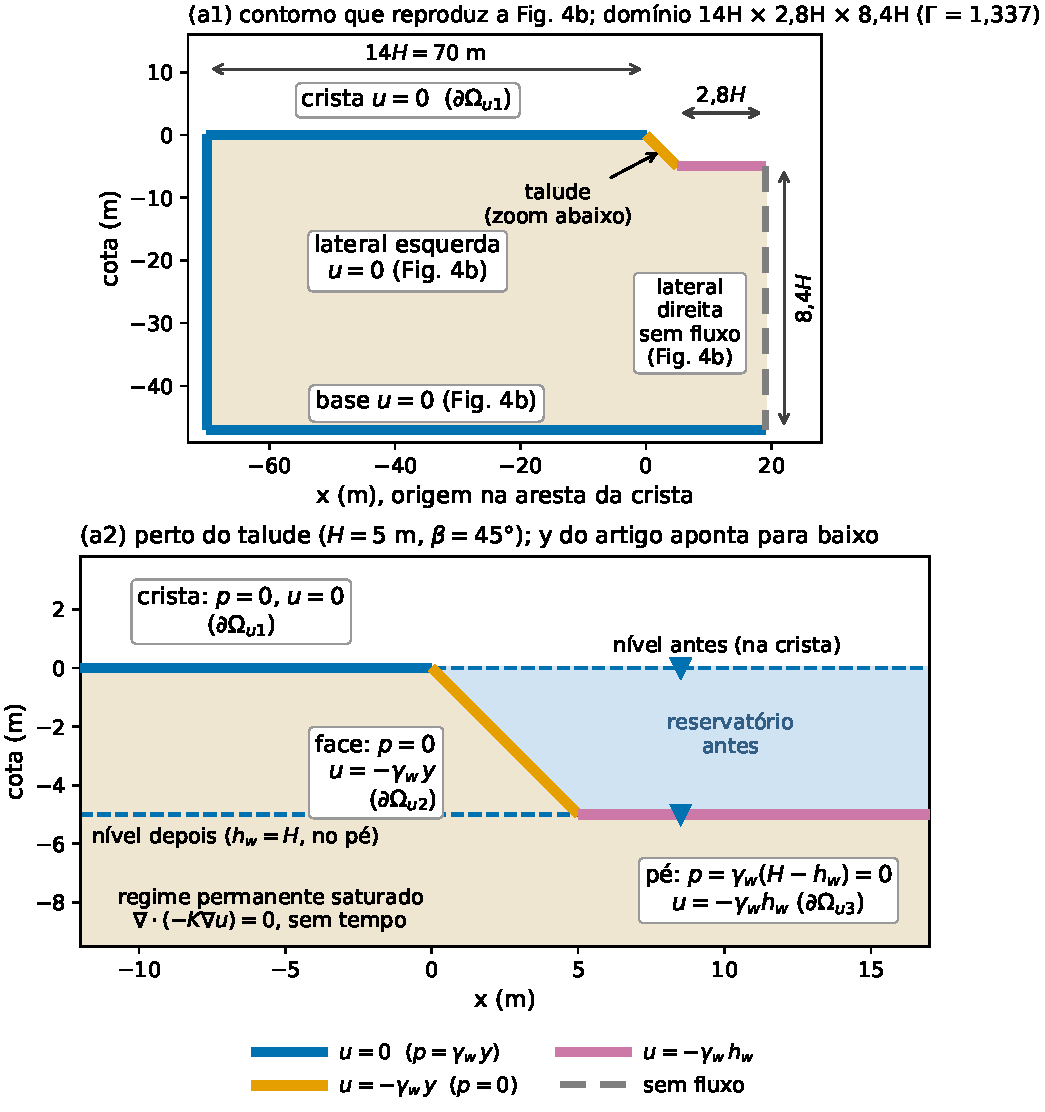
\includegraphics[width=\textwidth]{figs/esquema_a_ceron.pdf}
\caption{Ceron: o contorno da água permanente depois do rebaixamento instantâneo, em escala. (a1) O domínio
$14H \times 2{,}8H \times 8{,}4H$, o que dá $\Gamma = 1{,}337$ com este contorno; a Fig.~4b do artigo parece ter
$\sim 50H \times 10H \times 30H$. (a2) Perto do talude. Com $h_w = H$, a face fica inteira acima do nível final; se o
nível parasse acima do pé, a face abaixo do nível teria $u = -\gw h_w$ (rosa).}\label{fig:a}
\end{figure}

\subsection*{(b) PZ com o contorno \texttt{reservatorio} (o do nosso MC)}
Código: \path{Projects/SlopeRandomFieldRefinement/DrawdownTransient.h/.cpp} e \path{rebaixamento_mc.cpp}. É o
transiente só da água (esqueleto rígido, ar passivo), com a formulação u-pw-pa.
\begin{figure}[H]\centering
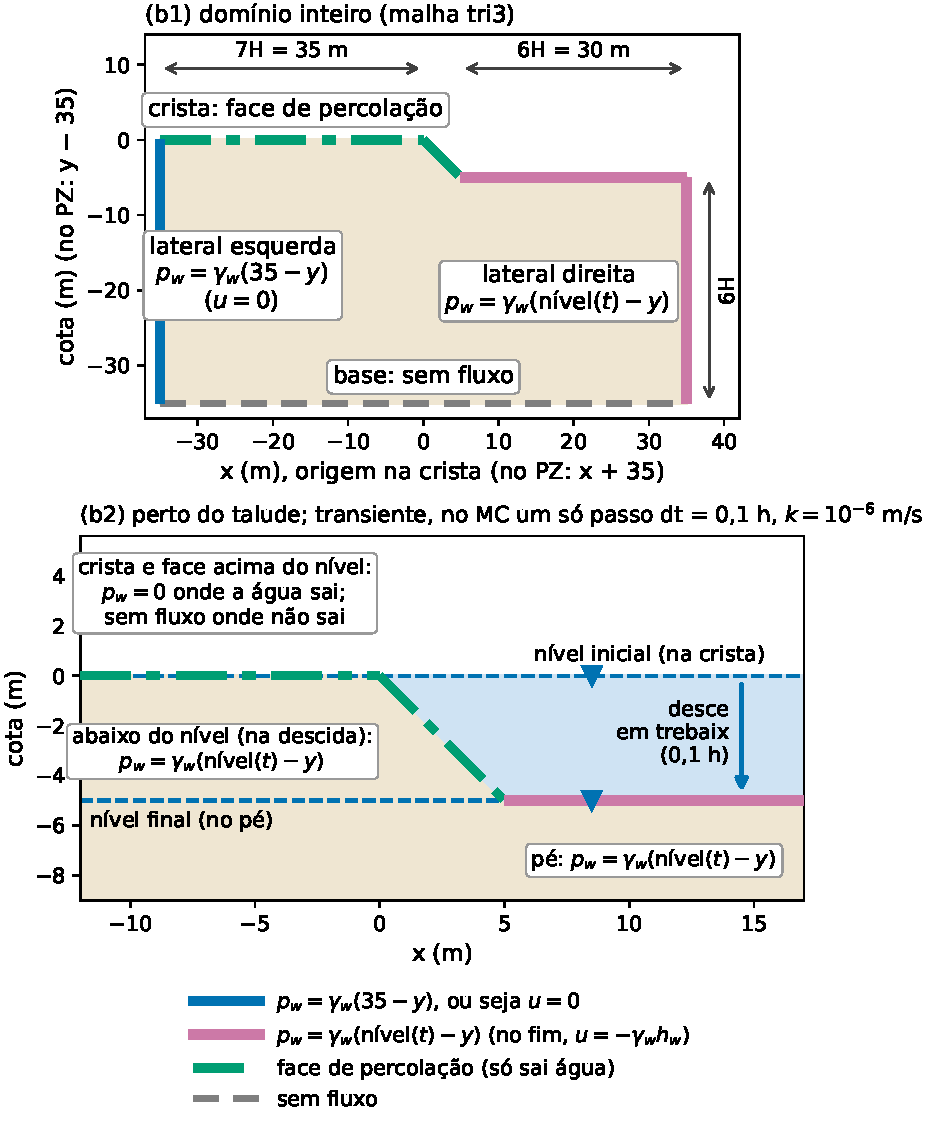
\includegraphics[width=\textwidth]{figs/esquema_b_pz_reservatorio.pdf}
\caption{PZ, contorno \texttt{reservatorio}: o lado do reservatório (lateral direita, pé, face e crista) tem a
hidrostática do nível do instante abaixo do nível e face de percolação acima (a água só sai). A base é sem fluxo e a
lateral esquerda fica hidrostática com o nível na crista. O nível desce linearmente em \texttt{trebaix}; no MC de
referência, $\texttt{trebaix} = \texttt{tfim} = \texttt{dt} = 0{,}1$~h, isto é, um passo só, com o nível final. O $k$
é $10^{-6}$~m/s, enquanto a Tab.~2 do artigo dá $k_v = 10^{-6}$~m$^4$/(kN\,s), ou seja $9{,}81\times10^{-6}$~m/s.}
\label{fig:b}
\end{figure}

\subsection*{(c) PZ com o contorno \texttt{ceron} (commit 4842ae2)}
\begin{figure}[H]\centering
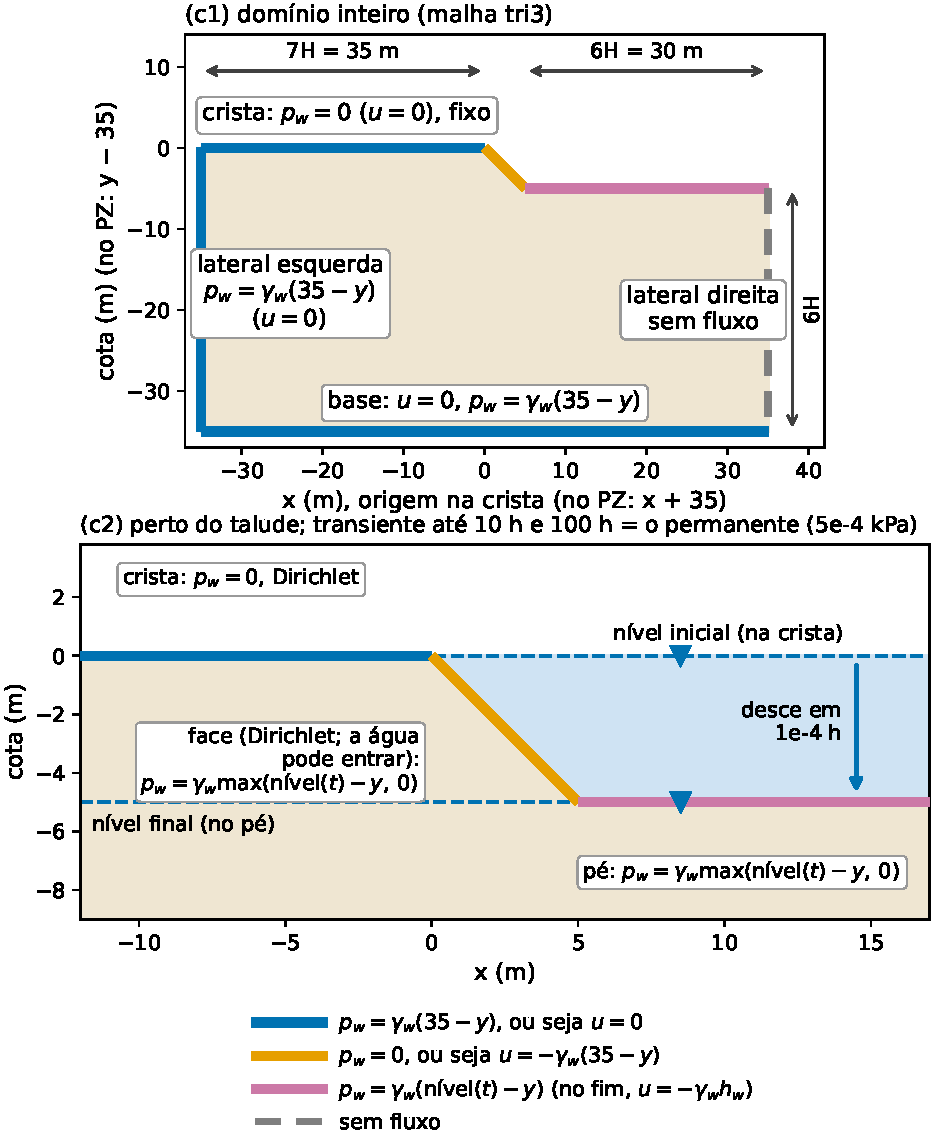
\includegraphics[width=\textwidth]{figs/esquema_c_pz_ceron.pdf}
\caption{PZ, contorno \texttt{ceron}: os contornos de (a), todos Dirichlet (a água pode entrar), com a lateral direita
sem fluxo. Rodado como rebaixamento instantâneo ($\texttt{trebaix} = 10^{-4}$~h) até 10~h e 100~h, o transiente
chega ao permanente: difere $5\times10^{-4}$~kPa (a precisão da exportação) de um Laplace independente na mesma
malha (Figura~\ref{fig:pzceron}). Como
$p_w \ge 0$ em todo o domínio, a água saturada e a não saturada dão o mesmo campo. Durante a descida, a face e o pé
usam o nível do instante; no regime final isso coincide com a Eq.~21.}\label{fig:c}
\end{figure}

\subsection*{(d) A chuva do Rahardjo como está no código}
Código, em \path{Projects/SlopeRandomFieldRefinement}: \path{rahardjo.cpp}, \path{montecarlo.cpp} e
\path{RainTransient.h/.cpp}.
Artigo: Rahardjo et al.\ (2007), Fig.~2 e págs.~1534--35 (o PDF está no Apêndice~\ref{sec:arquivos}).
\begin{figure}[H]\centering
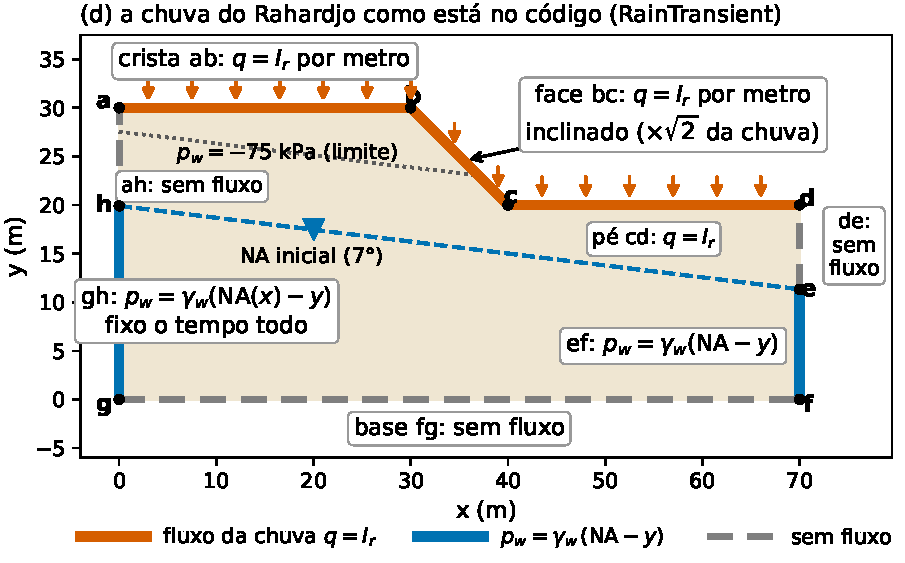
\includegraphics[width=\textwidth]{figs/esquema_d_rahardjo_codigo.pdf}
\caption{Rahardjo como está no código: talude de 45° e 10~m, NA a 5~m abaixo do pé, inclinado 7°. A chuva é um fluxo
$q = I_r$ na crista, na face e no pé, por 24~h. Se a chuva faz $p_w > 0$ num nó da superfície, o nó passa a $p_w = 0$
imposto (face de percolação) e o excesso escorre; o nó volta ao fluxo se absorveria mais que $q$. Depois de 24~h,
$q = 0$ e a face continua só deixando sair. Abaixo do NA, as laterais ficam com a hidrostática do NA inicial o tempo
todo; acima do NA e na base, sem fluxo. Estado inicial: $p_w = \max(\gw(\mathrm{NA} - y), -75~\mathrm{kPa})$
(pontilhado: onde chega a $-75$~kPa, 7,65~m acima do NA). Tudo isso confere com o artigo, menos a chuva na face
(D1) e o empoçamento (D2), que o artigo não descreve.}\label{fig:d}
\end{figure}

\subsection*{(e) O que muda na chuva nas etapas 4 e 5}
O código já segue o artigo em quase tudo (Tabela~\ref{tab:rahardjo}). Sobram decisões, não erros:
\begin{figure}[H]\centering
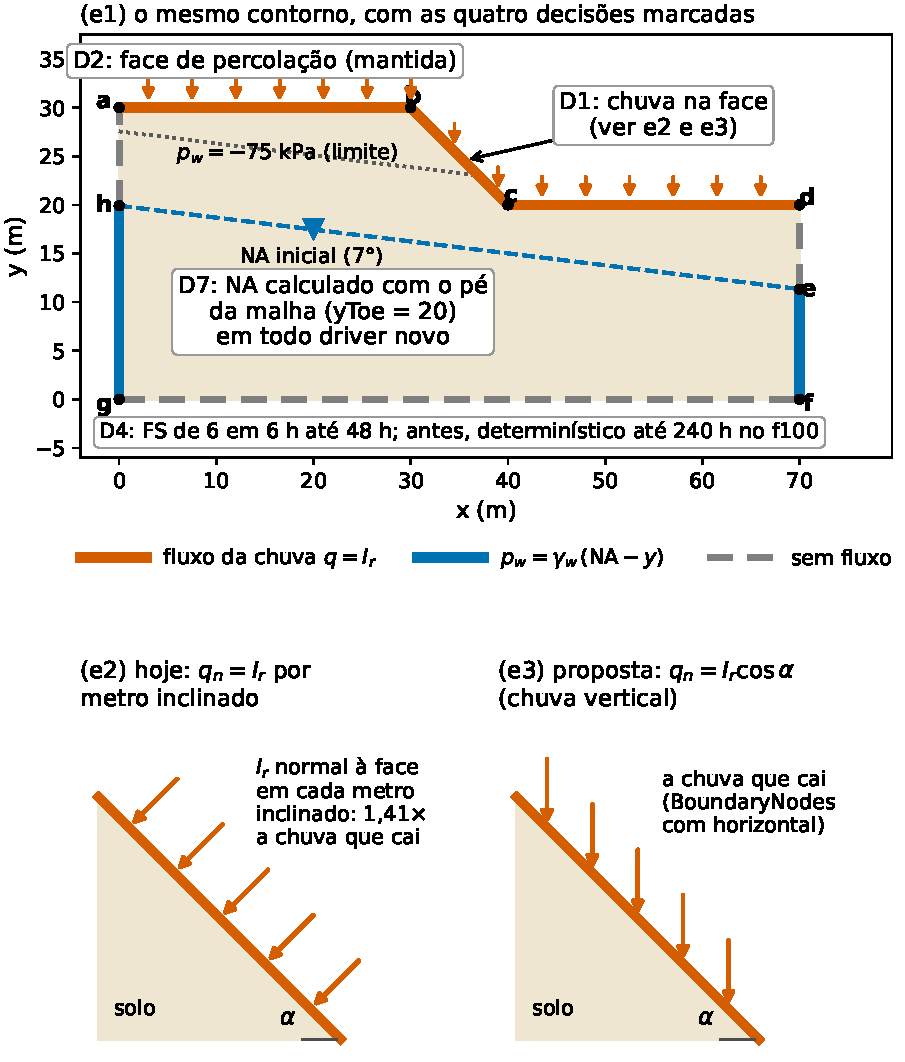
\includegraphics[width=\textwidth]{figs/esquema_e_rahardjo_plano.pdf}
\caption{O plano para a chuva. (e1) O contorno fica o mesmo de (d); as decisões estão marcadas. D1: a chuva na face
entra por metro inclinado (e2), 41\,\% a mais de água do que a chuva vertical (e3); a opção horizontal do
\texttt{BoundaryNodes} já existe e o \texttt{RainTransient} não a usa. D2: a face de percolação fica. D4: o artigo vai
até 240~h e nós, até 48~h. D7: o padrão do \texttt{RainData} (yToe = 30, da malha antiga) erra o NA em 10~m num driver
que não o sobrescreva.}\label{fig:e}
\end{figure}

\section{As tabelas dos contornos}
Tabelas~\ref{tab:unica} (rebaixamento) e \ref{tab:rahardjo} (chuva); linhas do código no commit 4842ae2.

\begin{landscape}
\footnotesize
\setlength{\tabcolsep}{4pt}\setlength{\LTcapwidth}{\linewidth}
\begin{longtable}{>{\raggedright}p{2.6cm}>{\raggedright}p{6.6cm}>{\raggedright}p{7.0cm}>{\raggedright\arraybackslash}p{6.4cm}}
\caption{Os contornos da água: Ceron (2025) $\times$ PZ \texttt{reservatorio} $\times$ PZ \texttt{ceron}. ``Fig.~4b''
quer dizer identificado reproduzindo a figura (não está no texto do artigo). DT = \texttt{DrawdownTransient.cpp};
RM = \texttt{rebaixamento\_mc.cpp}.}\label{tab:unica}\\
\toprule
Trecho & Ceron (artigo; e o identificado na Fig.~4b) & PZ \texttt{reservatorio} (padrão; MC de referência) & PZ \texttt{ceron} (commit 4842ae2) \\
\midrule\endfirsthead
\toprule
Trecho & Ceron & PZ \texttt{reservatorio} & PZ \texttt{ceron} \\
\midrule\endhead
\bottomrule\endfoot
Crista & $p = 0$, $u = 0$ (Eq.~1; Eq.~21 em $\partial\Omega_{u1}$) &
  Lado do reservatório (RM:994). Acima do nível para $t > 0$: face de percolação, $p_w = 0$ onde a água sai e sem fluxo
  onde não sai (DT:86--123). Na prática só drena e fica com sucção &
  $p_w = 0$ ($u = 0$), Dirichlet fixo (DT:28) \\ \midrule
Face acima do nível & $p = 0$, $u = -\gw y$ (Eq.~1; Eq.~21 em $\partial\Omega_{u2}$), Dirichlet &
  Face de percolação (o teste da crista, DT:92--113); onde $p_w = 0$ é imposto, $u = -\gw(35 - y)$. A água só sai &
  $p_w = \gw\max(\text{nível}(t) - y, 0) = 0$, ou seja $u = -\gw(35 - y)$; Dirichlet \emph{sem} o teste de saída: a
  água pode entrar (DT:69) \\ \midrule
Face abaixo do nível & $p = \gw(y - h_w)$, $u = -\gw h_w$ (Eq.~1; $\partial\Omega_{u3}$) &
  $p_w = \gw(\text{nível}(t) - y)$, Dirichlet (DT:89). No fim (nível 30), a face fica toda acima do nível &
  $p_w = \gw(\text{nível}(t) - y)$, Dirichlet (DT:69). No fim, $u = -\gw h_w = -49{,}05$~kPa \\ \midrule
Terreno do pé & $p = \gw(H - h_w)$, $u = -\gw h_w$ (Eq.~1; $\partial\Omega_{u3}$); com $h_w = H$: $p = 0$ e
  $u = -49{,}05$~kPa &
  $p_w = \gw(\text{nível} - y)$, Dirichlet (teste \texttt{y <= nivel}, DT:89). No fim, $p_w = 0$, $u = -49{,}05$~kPa &
  $p_w = \gw\max(\text{nível} - y, 0)$. No fim, $p_w = 0$, $u = -49{,}05$~kPa (DT:69) \\ \midrule
Lateral esquerda (maciço) & Não está no artigo. Fig.~4b: $u = 0$ ($p = \gw y$) &
  $p_w = \gw(35 - y)$ ($u = 0$), Dirichlet em toda a altura (DT:11--14; RM:988) &
  $p_w = \gw(35 - y)$ ($u = 0$), Dirichlet (DT:25--27) \\ \midrule
Lateral direita (reservatório) & Não está no artigo. Fig.~4b: \textbf{sem fluxo} (contradiz o
  $\partial\Omega_v = \emptyset$ literal, que pediria $u$ imposto também aqui; no contorno C, $u = -\gw h_w$) &
  $p_w = \gw(\text{nível}(t) - y)$, Dirichlet (lado do reservatório). No fim, $u = -\gw h_w$ &
  \textbf{Sem fluxo} (fora de \texttt{DrawdownCeronIds}; RM:993) \\ \midrule
Base & Não está no artigo. Fig.~4b: $u = 0$ ($p = \gw y$) & \textbf{Sem fluxo} (em nenhuma lista) &
  $p_w = \gw(35 - y)$ ($u = 0$), Dirichlet (DT:25--27) \\ \midrule
Estado inicial & Hidrostático com o nível na crista: $u = 0$ (texto da Eq.~2) &
  Hidrostático com o nível na crista (DT:39--48; RM:986) & O mesmo (\texttt{InitialState} comum) \\ \midrule
Tempo & \textbf{Permanente} logo depois do rebaixamento \textbf{instantâneo}; sem armazenamento; no homogêneo o $k$
  não importa &
  \textbf{Transiente} (Euler implícito; armazenamento $n/K_w$; van Genuchten no \texttt{agua=unsat}). Nível descendo
  linearmente em \texttt{trebaix}; no MC, $\texttt{trebaix} = \texttt{tfim} = \texttt{dt} = 0{,}1$~h: um passo só,
  com o nível final (DT:50--62). $k = 10^{-6}$~m/s, contra $9{,}81\times10^{-6}$~m/s da Tab.~2 &
  Transiente rodado como instantâneo ($\texttt{trebaix} = 10^{-4}$~h) até o regime: 10~h (dt 0,5) e 100~h (dt 1).
  Bate com o permanente P1 independente a $5\times10^{-4}$~kPa; $p_w \ge 0$, então sat = unsat \\ \midrule
Domínio & Medido na Fig.~4b: $\sim 50H$ atrás da crista, $10H$ à frente do pé, $30H$ abaixo do pé &
  $7H \times 6H \times 6H$ (malha tri3) & $7H \times 6H \times 6H$ (malha tri3) \\
\end{longtable}
\end{landscape}

\begin{landscape}
\footnotesize
\setlength{\tabcolsep}{4pt}\setlength{\LTcapwidth}{\linewidth}
\begin{longtable}{>{\raggedright}p{2.5cm}>{\raggedright}p{5.6cm}>{\raggedright}p{7.6cm}>{\raggedright\arraybackslash}p{6.9cm}}
\caption{A chuva do Rahardjo: o artigo (2007) $\times$ o código de hoje $\times$ o que vamos fazer nas etapas 4 e 5.
D1--D7 são as divergências da Figura~\ref{fig:e}. RT = \texttt{RainTransient.cpp}; RH = \texttt{rahardjo.cpp}; MC =
\texttt{montecarlo.cpp}. ``Proposta'' marca o que ainda não foi decidido.}\label{tab:rahardjo}\\
\toprule
Item & Artigo & Código hoje & O que vamos fazer \\
\midrule\endfirsthead
\toprule
Item & Artigo & Código hoje & O que vamos fazer \\
\midrule\endhead
\bottomrule\endfoot
Geometria & $H_s = 10$~m, $\alpha = 45^\circ$; crista, pé e lateral esquerda $3H_s$, direita $2H_s$ (Fig.~2) &
  $\{(0,0),(70,0),(70,20),(40,20),(30,30),(0,30)\}$ (RH:282; MC:104) & igual \\ \midrule
NA inicial & 5~m abaixo do pé, 7° subindo para dentro do maciço &
  \texttt{WaterLevel(x)} com yToe = 20 e xToe = 40 vindos dos drivers: 19,91~m em $x = 0$; 11,32~m em $x = 70$.
  O padrão do \texttt{RainData} é yToe = 30 (malha antiga) &
  D7 (proposta): todo driver novo passa yToe e xToe da malha; trocar o padrão evita o erro de 10~m \\ \midrule
Crista, face e pé (ab, bc, cd) & ``$q = I_r$'' na superfície &
  Vazão nodal $q\,L$, com $L$ = metade de cada aresta \emph{inclinada} (RT:16--18, 59;
  \texttt{TPZUnsatAnalysis::BoundaryNodes}, \texttt{Analysis/TPZUnsatAnalysis.cpp}:116--129) &
  \textbf{D1} (proposta): chuva vertical, $q_n = I_r\cos\alpha$ na face (\texttt{BoundaryNodes(id, true)}); medir antes
  o efeito no FS mínimo (determinístico, f50 e f100, 80~mm/h) \\ \midrule
Superfície com $p_w > 0$ & não diz (só ``shed off as runoff'') &
  Face de percolação com escoamento: $p_w = 0$ imposto; volta ao fluxo se absorveria mais que $q$; até 40 iterações
  (RT:48--85) & \textbf{D2}: manter (registrar como hipótese nossa) \\ \midrule
Depois de 24~h & não diz & $q = 0$; a face continua só deixando sair; chuva proporcional no passo que cruza 24~h
  (RT:39--40) & manter \\ \midrule
Evaporação & só no esquema da Fig.~1 & não há & igual \\ \midrule
Laterais acima do NA (ah, de) & $Q = 0$ & sem fluxo (só os nós com $y \le$ nível são impostos, RT:11--15) & igual \\ \midrule
Laterais abaixo do NA (gh, ef) & carga total do NA inicial & $p_w = \gw(\text{nível}(x) - y)$ fixo o tempo todo
  (RT:11--15) & igual \\ \midrule
Base (fg) & $Q = 0$ & sem fluxo & igual \\ \midrule
Estado inicial & hidrostático com limite de $-75$~kPa & $p_w = \max(\gw(\text{nível} - y), -75)$ (RT:21--25). Não
  é permanente (NA inclinado, sucção cortada): há fluxo sem chuva, como no SEEP/W & igual \\ \midrule
Solo & Fredlund--Xing ($n = m = 1$, $\theta_s = 0{,}45$, $a$ = 10/50/100~kPa); $k = k_s\Theta^4$;
  $k_s$ = 1e-4/1e-5/1e-6~m/s & \texttt{EFredlundXing}, \texttt{EPowerLaw} $\Theta^4$, porosidade 0,45 & igual \\ \midrule
Armazenamento & $m_2^w\gw$ (inclinação da SWCC) & $n\,dS_w/dp_c$ \emph{mais} $n/K_w$ ($K_w = 2{,}2\times10^6$~kPa),
  concentrado & \textbf{D3}: manter; medir uma vez sem $K_w$ (opcional) \\ \midrule
Acoplamento & SEEP/W desacoplado, $p_w$ exportada para o SLOPE/W &
  u-pw-pa com esqueleto rígido ($u = 0$) e ar passivo ($p_a = 0$) no transiente (RT:9--10; RH:119; MC:406) &
  proposta: manter como caso base (é o desacoplado do artigo); o acoplado fica como variação \\ \midrule
Resistência & $c' = 10$, $\phi' = \phi^b = 26^\circ$, $\gamma = 20$ & $\chi = 1$; $\gamma = 20$; $E = 2\times10^4$,
  $\nu = 0{,}3$ (nossos) & igual \\ \midrule
FS & Bishop simplificado (SLOPE/W) & SRM ou GIM com $p_w$ congelada; base presa, laterais presas em $x$.
  FS inicial 2,10 nos três solos (README, etapa 5); o 2,118 que o RH:273 imprime é o valor do artigo & \textbf{D5}: diferença esperada; registrar \\ \midrule
Malha e passo & não dados & transiente: H/8 = 1,25~m (RH) e H/4 = 2,5~m (MC); dt = 0,1~h; FS: TriGMesh(1) + 4 níveis
  & \textbf{D6} (proposta): conferir no determinístico se 2,5~m basta; usar a mesma malha nos dois drivers \\ \midrule
Horizonte & curva até 240~h (Fig.~4) & até 48~h (RH, de hora em hora); no MC, \texttt{tempos=} na linha de comando (padrão 0 e 24~h; nas campanhas, de
  6 em 6~h até 48~h) &
  \textbf{D4}: determinístico até 240~h no f100; se o mínimo passar de 48~h, ampliar \texttt{tempos} \\ \midrule
Chuvas & 13 intensidades por 24~h; série A: 9, 80 e $1\,k_s$ & \texttt{I=} pela linha de comando (padrão $1\,k_s$) &
  9 e 80~mm/h nos três solos (etapa 5) \\
\end{longtable}
\end{landscape}

\section{Resultados já obtidos}
Todos são determinísticos (sem campo aleatório), com $c' = 10$~kPa, $\phi' = 30^\circ$, $\gamma = 20$~kN/m$^3$. Os dados
estão em \path{Projects/CeronCinematico/dados} e as rodadas do PZ em \path{~/projects/runs/ceron_contorno} e
\path{~/projects/runs/ceron_instantaneo}. As figuras originais do \path{Projects/CeronCinematico/figs} estão copiadas em
\path{figs/}; no texto entram painéis recortados (Seção~\ref{sec:fig4}) ou figuras redesenhadas aqui com os mesmos
dados, para a fonte ficar legível.

\subsection{A Fig.~4 do Ceron reproduzida}\label{sec:fig4}
O painel D (Figura~\ref{fig:4b}) mostra que, com lateral esquerda e base em $u = 0$ e lateral direita sem fluxo, as
nossas isolinhas (vermelho) caem sobre as da Fig.~4b (cinza) no domínio medido na figura. Os outros três contornos
testados (B, C e um quarto com a base também sem fluxo) não batem; estão em \path{figs/fig4b_reproducao.png}. A
Figura~\ref{fig:4c} compara as forças de percolação $-\nabla u$ com a Fig.~4c.

\begin{landscape}
\begin{figure}[p]\centering
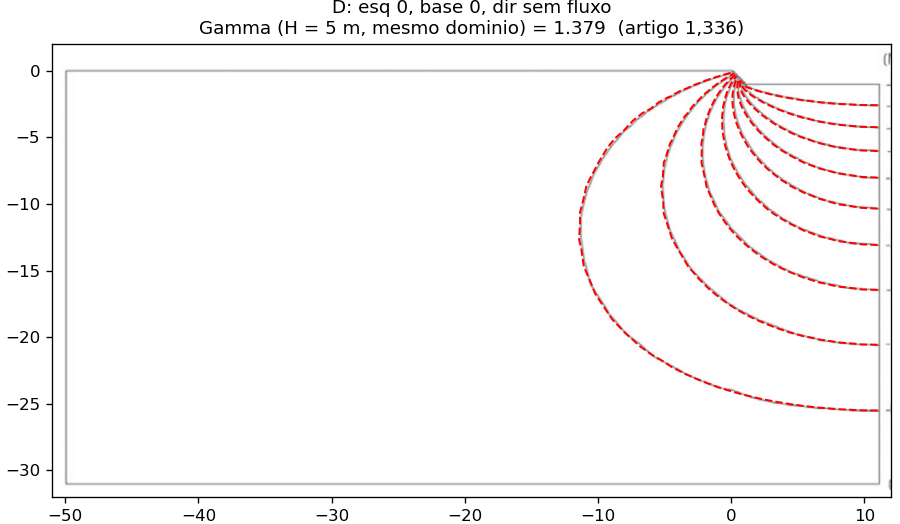
\includegraphics[width=0.95\linewidth]{figs/fig4b_painel_D.png}
\caption{Fig.~4b do Ceron (cinza, a imagem do artigo) e as nossas isolinhas de $u$ (vermelho tracejado), de
$-0{,}1$ a $-0{,}9\,\gw h_w$, com lateral esquerda e base $u = 0$ e lateral direita sem fluxo, no domínio
$50H \times 10H \times 30H$ ($x$ e cota em unidades de $H$, como na figura do artigo: o talude é o trecho de 0 a 1
perto da origem). Com este domínio e $H = 5$~m, $\Gamma = 1{,}379$ (o ``Gamma'' do título). Painel D de
\texttt{figs/fig4b\_reproducao.png} (\texttt{Projects/CeronCinematico/fig4b\_ceron.py}).}\label{fig:4b}
\end{figure}
\end{landscape}

\begin{landscape}
\begin{figure}[p]\centering
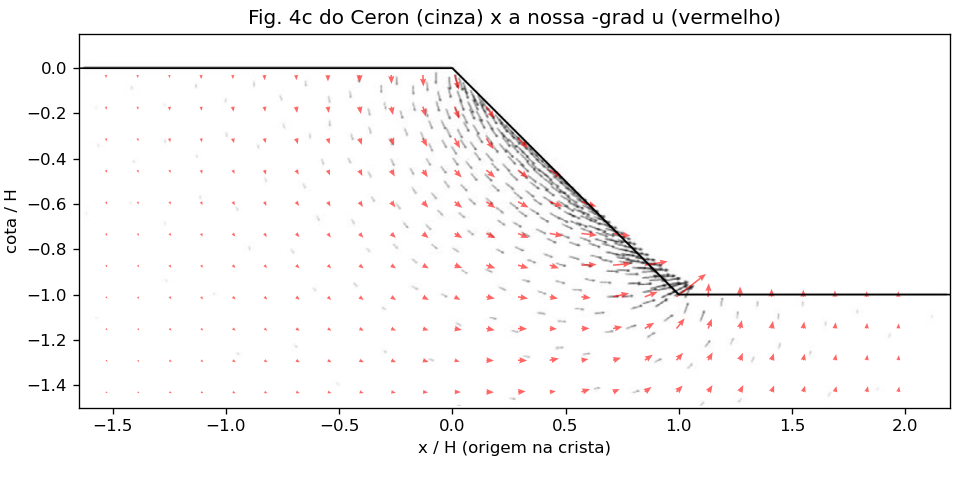
\includegraphics[width=0.95\linewidth]{figs/fig4c_painel_esq.png}
\caption{Fig.~4c do Ceron (cinza) e a nossa $-\nabla u$ (vermelho), com o contorno da Figura~\ref{fig:4b} e domínio
$14H \times 2{,}8H \times 8{,}4H$. As direções coincidem, inclusive o fluxo saindo pela face e subindo no pé. Painel
esquerdo de \texttt{figs/fig4c\_reproducao.png} (\texttt{Projects/CeronCinematico/fig4c\_ceron.py}).}\label{fig:4c}
\end{figure}
\end{landscape}

\subsection{O $\Gamma$ depende do contorno e do domínio}\label{sec:dominio}
Água permanente saturada (Eqs.~19--21), malha própria P1 e $\Gamma$ cinemático
(\path{estudo_contorno.py}, em \path{Projects/CeronCinematico}). Os quatro contornos testados:
\begin{itemize}
  \item \textbf{A:} só crista, face e pé impostos; laterais e base sem fluxo (a célula 1 do notebook do Mário);
  \item \textbf{B:} A mais lateral esquerda $u = 0$ e direita $u = -\gw h_w$, base sem fluxo (célula 9);
  \item \textbf{C:} tudo Dirichlet ($\partial\Omega_v = \emptyset$ literal): esquerda e base 0, direita $-\gw h_w$;
  \item \textbf{D:} esquerda e base $u = 0$, direita sem fluxo (o que reproduz a Fig.~4b).
\end{itemize}

\begin{figure}[H]\centering
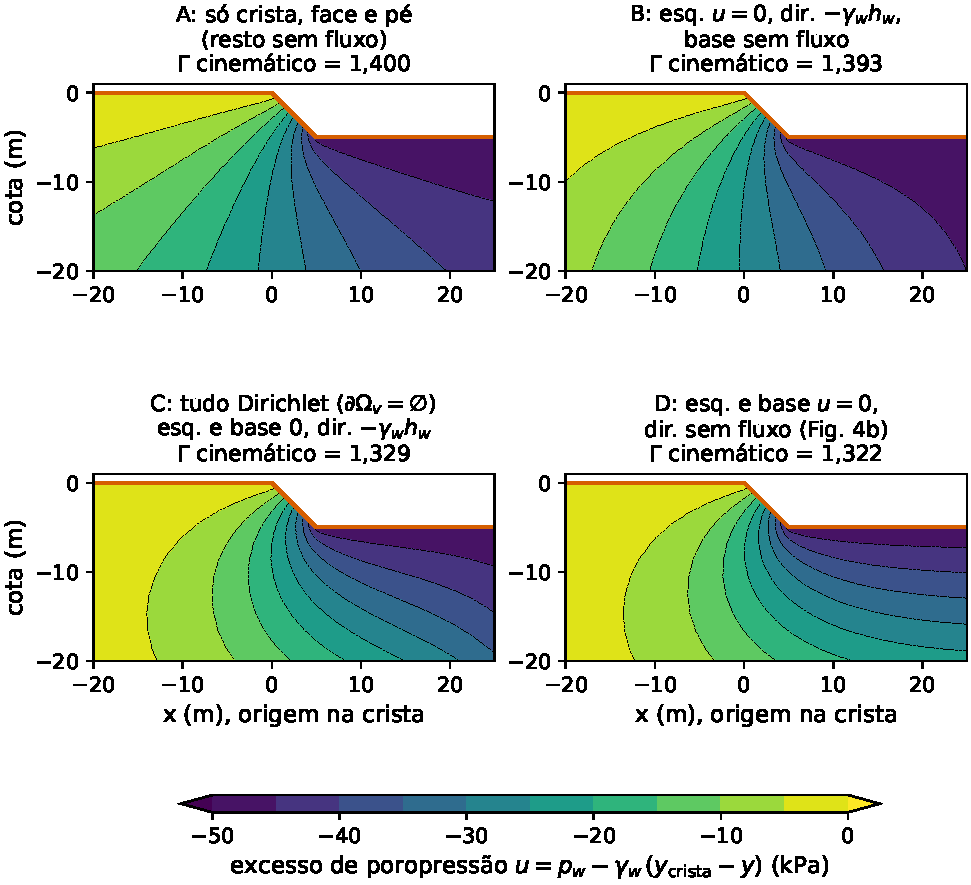
\includegraphics[width=\textwidth]{figs/permanente_contornos.pdf}
\caption{O excesso de poropressão permanente com os contornos A a D, no nosso domínio $7H \times 6H \times 6H$ (zoom
perto do talude). O que muda é a água longe do talude: com a base sem fluxo (A, B), o maciço inteiro drena para o
pé e $u$ fica negativo atrás da crista; com a base em $u = 0$ (C, D), a base repõe água, $u$ fica perto de 0 atrás da
crista e o $\Gamma$ cai uns 5\,\%.}
\label{fig:perm}
\end{figure}

\begin{table}[H]\centering
\caption{$\Gamma$ cinemático com a água permanente, por domínio e contorno (\texttt{dados/estudo\_contorno.csv}). O
artigo dá 1,336.}\label{tab:dominio}
\tabdominio
\end{table}

\begin{figure}[H]\centering
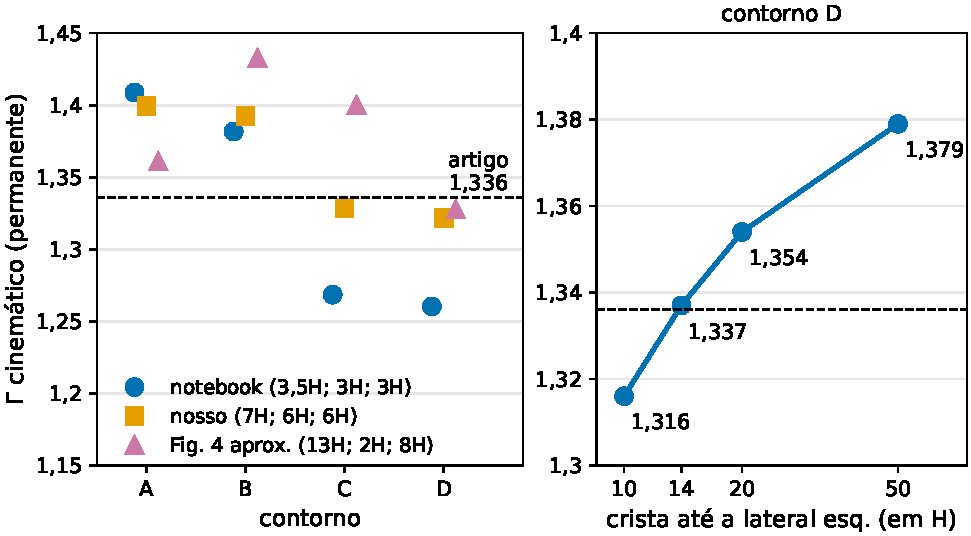
\includegraphics[width=\textwidth]{figs/gamma_dominio.pdf}
\caption{Esquerda: a Tabela~\ref{tab:dominio} em gráfico; o contorno pesa até $\pm 7\,\%$ e o domínio muda até a
ordem dos contornos. Direita: com o contorno D, o $\Gamma$ cresce com o domínio, 1,316 ($10H$), 1,337 ($14H \times
2{,}8H \times 8{,}4H$), 1,354 ($20H$) e 1,379 ($50H$, o da Fig.~4b); o 1,336 do artigo corresponde a $\sim 14H$
(README, etapa 3d, passo 1b). Na Figura~\ref{fig:4b}, o domínio de 50H reproduz as isolinhas, mas dá 1,379: o
domínio do $\Gamma$ do artigo não é, necessariamente, o da figura.}\label{fig:gdom}
\end{figure}

\subsection{PZ \texttt{reservatorio}: o rebaixamento instantâneo}
Para separar o efeito do tempo do efeito dos contornos, rodamos o contorno \texttt{reservatorio} com o rebaixamento
instantâneo ($\texttt{trebaix} = 10^{-4}$~h) e olhamos $t = 0^+$, 0,1, 1 e 10~h
(\path{dados/instantaneo_pz.csv}, \path{dados/rodar_instantaneo.sh}).

\begin{figure}[H]\centering
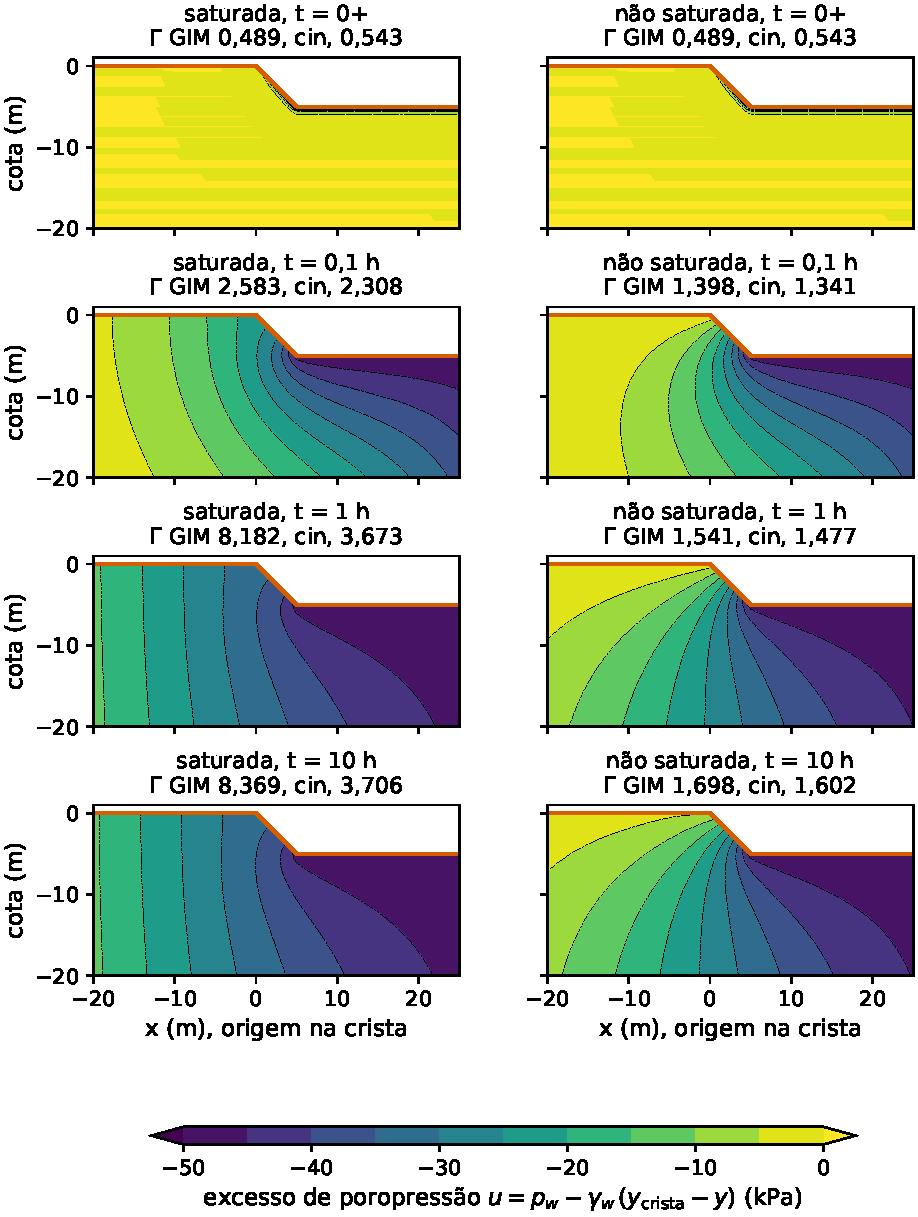
\includegraphics[width=\textwidth]{figs/instantaneo_campos.pdf}
\caption{PZ, contorno \texttt{reservatorio}, rebaixamento instantâneo. Esquerda: água saturada; direita: não
saturada. Em $t = 0^+$ a água ainda não se moveu ($u \approx 0$ em quase todo o domínio, $\Gamma = 0{,}49$). Com a
água saturada, $u$ cai em todo o maciço já em 1~h: o $\Gamma$ do GIM vai a 8,2 (1~h) e 8,4 (10~h), e o cinemático a
3,7. Com a não
saturada, a água sai mais devagar (provavelmente porque o $k$ cai com a sucção perto da superfície) e o $\Gamma$ vai
de 1,40 (0,1~h) a 1,70 (10~h). Nenhum instante tem a água do Ceron (Figura~\ref{fig:perm}, D).}\label{fig:inst}
\end{figure}

Na água saturada de 1 e 10~h, o GIM (8,2 e 8,4) fica bem acima do cinemático (3,7), que é limite superior. Os dois
não medem a mesma coisa: o GIM multiplica só o peso (e a água do reservatório) e deixa $p_w$ congelada, inclusive a
sucção; o cinemático multiplica o peso \emph{e} as forças de percolação $-\nabla u$ (\path{cinematico.py}, Eq.~54).
Com $\Gamma \approx 1{,}3$ e pouca sucção os dois concordam (Tabela~\ref{tab:gamma}); com sucção forte, não. A causa
exata não foi investigada.

\begin{table}[H]\centering
\caption{$\Gamma$ do rebaixamento instantâneo com o contorno \texttt{reservatorio} (GIM com 3 níveis e cinemático).
O u-p e o u-pw-pa dão o mesmo $\Gamma$ até a 3.ª casa. Passos de tempo: $10^{-4}$, 0,01, 0,1 e 0,5~h
(\texttt{\textasciitilde/projects/runs/ceron\_instantaneo/rodar.sh}).}\label{tab:inst}
\tabinstantaneo
\end{table}

\subsection{PZ \texttt{ceron}: a água do Ceron dentro do PZ}
\begin{figure}[H]\centering
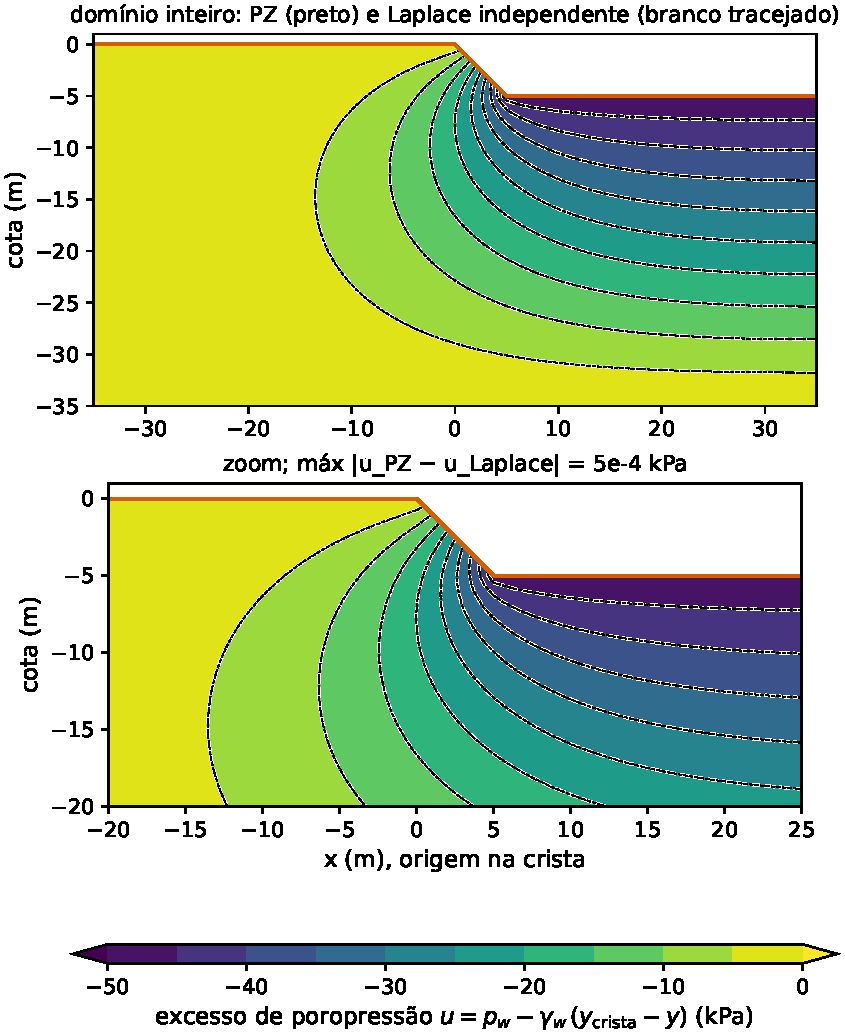
\includegraphics[width=\textwidth]{figs/pz_ceron_campo.pdf}
\caption{PZ com \texttt{contorno=ceron}, água saturada em $t = 10$~h (as rodadas não saturadas em 10~h e 100~h dão o
mesmo campo). As isolinhas do PZ (preto) e as do Laplace independente com o contorno D na mesma malha (branco
tracejado) coincidem: a diferença máxima é $5\times10^{-4}$~kPa (\texttt{dados/pz\_contorno\_ceron.csv}), que é a precisão da
exportação ($p_w$ gravada com 6 algarismos). A comparação é na \emph{mesma} malha (tri3, lado de 0,625~m).}
\label{fig:pzceron}
\end{figure}

\begin{figure}[H]\centering
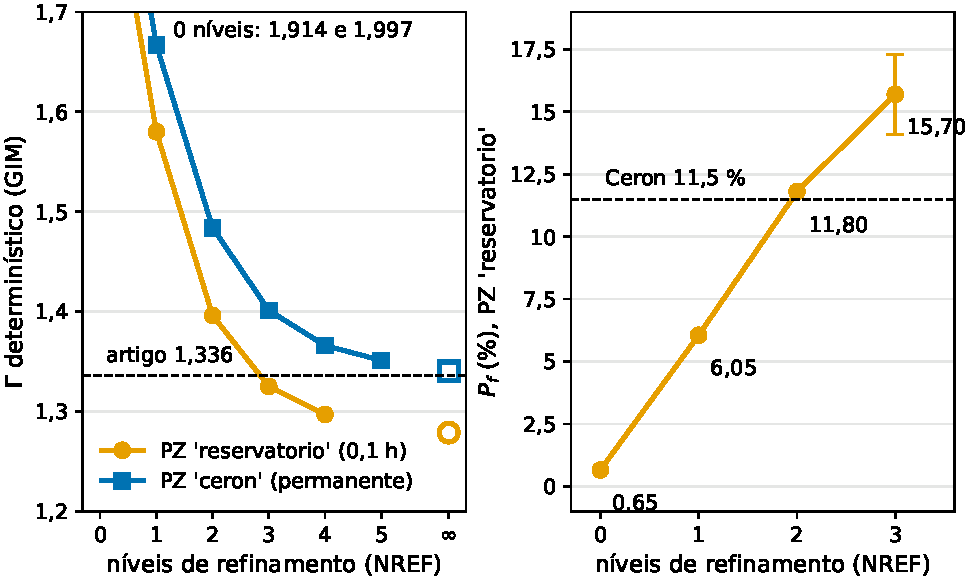
\includegraphics[width=\textwidth]{figs/convergencia.pdf}
\caption{Esquerda: $\Gamma$ do GIM contra o número de níveis de refinamento. Com a nossa água de 0,1~h
(\texttt{reservatorio}, laranja), o $\Gamma$ cai abaixo do 1,336 a partir de 3 níveis e vai a $\approx 1{,}28$ (círculo
vazio, extrapolado com 2, 3 e 4 níveis). Com a água do Ceron (\texttt{ceron}, azul), vai a \gextceron{} (quadrado
vazio, Richardson com 3, 4 e 5 níveis, razão 0,42); os dois partem de malhas grossas parecidas (0 níveis: 1,914 e
1,997). Direita: a $P_f$ do MC de referência (\texttt{reservatorio}) ainda
cresce com o refinamento; com 2 níveis já está no 11,5\,\% do Ceron e, com 3, acima.}\label{fig:conv}
\end{figure}

\begin{table}[H]\centering
\caption{Resumo do $\Gamma$ determinístico. ``Extrap.'' = Richardson com os três últimos níveis. Fontes: README
(etapa 3d), \texttt{dados/pz\_contorno\_ceron.csv}, \texttt{\textasciitilde{}/projects/runs/ceron\_contorno/sat\_ceron\_n4\_0\_-1.csv} e
\texttt{sat\_ceron\_n5\_0\_-1.csv} (coluna dos níveis), \texttt{padrao\_0\_-1.csv}, \texttt{CeronCinematico/README.md}.}\label{tab:gamma}
\small
\setlength{\tabcolsep}{4.5pt}
\begin{tabular}{lrrrrrrr}\toprule
 & \multicolumn{4}{c}{GIM, NREF} & & & \\ \cmidrule(lr){2-5}
Água & 2 & 3 & 4 & 5 & extrap. & cinemático & artigo \\ \midrule
PZ \texttt{reservatorio}, 0,1~h (MC) & 1,396 & 1,325 & 1,297 & --- & $\approx 1{,}28$ & 1,279$^a$ & 1,336 \\
PZ \texttt{reservatorio}, \texttt{det} & \gdetii & 1,3253 & 1,2973 & 1,2851 & 1,276 & 1,279 & 1,336 \\
PZ \texttt{ceron}, permanente & \gcerii & \gceriii & \gceriv & \gcerv & \gextceron & \gcin & 1,336 \\
Python, D, $7H \times 6H \times 6H$ & --- & --- & --- & --- & --- & 1,322$^b$ & 1,336 \\
Python, D, $14H \times 2{,}8H \times 8{,}4H$ & --- & --- & --- & --- & --- & 1,337 & 1,336 \\
\bottomrule\end{tabular}

\smallskip
{\footnotesize $^a$ na exportação \texttt{det} da mesma água. $^b$ malha própria com $h = 0{,}125$~m perto do
talude; com $h = 0{,}0625$~m, \gpyfino.}
\end{table}

\paragraph{Leitura.}
\begin{itemize}
  \item Com a água do Ceron (na malha tri3), o PZ chega a \gextceron{} e o cinemático a \gcin{}: a 0,3--0,5\,\% do
    1,336 (mas veja o ponto em aberto abaixo). Com a nossa
    água de 0,1~h, chega a 1,28 ($-4\,\%$). A diferença de $P_f$ (15,7 contra 11,5\,\%) é compatível com isso:
    uma água ``pior'' e um refinamento que ainda não convergiu.
  \item \textbf{Ponto em aberto, em parte explicado:} o PZ \texttt{ceron} no nosso domínio ($7H$) dá \gcin{} no
    cinemático, mas o permanente em Python no mesmo domínio e com o mesmo contorno dá 1,322 (\gpyfino{} com a malha
    própria mais fina). Os $5\times10^{-4}$~kPa comparam o PZ com o Laplace na \emph{mesma} malha tri3; contra o
    Laplace na malha própria fina, o $u$ do PZ difere até \dufino~kPa. Levando o $u$ fino para a malha do PZ, o
    cinemático na malha do PZ dá \gpzufino{} (função \texttt{malha\_agua} do gerador). Então a maior parte da
    diferença vem da \emph{discretização da água} na malha tri3 (lado de 0,625~m, grossa perto da crista e do pé), e só
    uma parte pequena vem da malha da integração. Consequência: o \gcin{} e, provavelmente, o \gextceron{} do GIM
    (mesma água tri3) estão alguns milésimos a 1\,\% acima do que dariam com a água convergida. Falta medir o GIM com
    uma malha de água mais fina.
\end{itemize}

\section{Próximos passos}
\begin{enumerate}
  \item \textbf{MC com a água do Ceron, em Python} (\path{Projects/CeronCinematico}): a água permanente com o contorno
    D, os campos aleatórios do artigo e o $\Gamma$ cinemático. O piloto de 200 realizações está rodando; depois, as
    10\,000. Critério: $P_f \approx 11{,}5\,\%$ (CoV 2,77\,\%).
  \item \textbf{MC no PZ com \texttt{contorno=ceron}} e \texttt{nref=5}: o mesmo problema pelo MEF (GIM). Esperado:
    $P_f$ um pouco acima da do cinemático, que é limite superior em cada realização. O domínio ($7H$ contra
    $\sim 14H$) e o $k$ (Tab.~2) ficam registrados como diferenças.
  \item \textbf{Escolher o domínio:} decidir se o MC de referência usa o $7H$ (o da malha atual) ou o de $14H$
    (o que dá 1,337). Pela Figura~\ref{fig:gdom}, a escolha muda o $\Gamma$ em 1--2\,\%.
  \item \textbf{A chuva (etapas 4 e 5):} decidir D1 (chuva por metro inclinado ou vertical) com um determinístico, e
    D4 (o horizonte) com um determinístico até 240~h no f100; depois, a linha 0 da etapa 5 (\texttt{rahardjo.cpp
    <solo> <I\_r> 48}, 3 solos $\times$ 2 chuvas) e as chaves que faltam no \path{montecarlo.cpp} (\texttt{xi=},
    \texttt{desloc\_xi=}, \texttt{gradiente=K}).
\end{enumerate}

\appendix
\section{Arquivos}\label{sec:arquivos}
\begin{itemize}
  \item Este documento: \path{Projects/PlanoDeTrabalho/contornos_agua/} (\path{gera.sh} refaz tudo;
    \path{figuras_contornos.py} só lê o \path{Projects/CeronCinematico} e as rodadas).
  \item Cópias das figuras originais em \path{figs/}: \path{fig4b_reproducao}, \path{fig4c_reproducao},
    \path{pressao_permanente}, \path{instantaneo_pz} e \path{pz_contorno_ceron} (.png e .pdf). As três últimas foram
    redesenhadas aqui (Figuras~\ref{fig:perm}, \ref{fig:inst} e \ref{fig:pzceron}) com os mesmos dados.
  \item Ceron (2025): \path{~/Num Anal Meth Geomechanics - 2025 - Vargas Ceron - ...pdf}, Eqs.~1, 2, 19--21, Figs.~2
    e 4, Tab.~2 e Fig.~24.
  \item Rahardjo et al.\ (2007): \path{~/Dropbox/UnsaturatedSoil/referencias/referencias_selecionadas_claude/Rahardjo_2007_JGGE.pdf}, Fig.~2, Eqs.~1--5,
    Tab.~1, ``Seepage Analysis'' e Fig.~4.
\end{itemize}
\end{document}
